\documentclass[pageno]{jpaper}
\usepackage{multirow}
\usepackage{adjustbox}
\usepackage[]{geometry}
\usepackage{changepage}
% to be able to draw some self-contained figs
\usepackage{tikz}
\usepackage{amsmath}
\usepackage{wrapfig}
\usepackage{color}

%replace XXX with the submission number you are given from the ASPLOS submission site.
\newcommand{\asplossubmissionnumber}{XXX}

\usepackage[normalem]{ulem}

\begin{document}

\title{
Instructions for Submission to ASPLOS 2021}

\date{}
\maketitle

\thispagestyle{empty}

\begin{abstract}

This document is intended to serve as a sample for submissions to the
26th International Conference on Architectural Support for Programming
Languages and Operating Systems (ASPLOS), 2021.  It provides
guidelines that authors should follow when submitting papers to the
conference. 
\end{abstract}

\label{sec:intro}
There are benefits to slowing down network driven workloads.

Two types of slowing down:
\begin{itemize}
    \item Slow down when to process packets from NIC
    \item Slow down processor clock speed
\end{itemize}

How do application behave under two types of network driven workloads:
\begin{itemize}
    \item Close-loop: Increase utilization of machines during diurnal troughs, the system controls the amount of admitted work. Faster time to completion == lower energy
    \item Open-loop: Focused on tail latency combined with SLA objectives
\end{itemize}

What are the types of benefits:
\begin{itemize}
    \item A combination of lower time + lower energy to complete some fixed work + (trade-offs that exist within this combination)
    \item A combination of tail latency + lower energy while meeting SLA objectives + (trade-offs that exist within this combination)
\end{itemize}

How is slowing down beneficial dependent on OS structure (os path length):
\begin{itemize}
    \item Linux - monolithic kernel, interrupt driven
    \item LibOS - unikernel, run-to-completion
\end{itemize}

Further questions and discussions:
\begin{itemize}
    \item Race-to-halt vs slowing down. Right now it is heuristics/black box, can this paper help to say when you should do this and why?
    \item Why is this benefit useful for the system policy designer/os designer? You should do this or that
    \item If we care about performance, why not just poll? Why is polling not enough?
    \item Having different ways to trade off performance+energy is a useful tool to have
\end{itemize}

% There are benefits to slowing down network driven processing.

% Race-to-halt vs slowing down. Right now it is heuristics/black box, can this paper help to say when you should do this and why?

% Two ways to slow down:
% 1) Delay when to process packets, 2)Slow down processor speed

% Two types of network driven workloads + justifying this:
% Close-loop - Netpipe, NodeJS web server
% Open-loop - Memcached, Memcached-Silo

% Types of benefit: 
% Lower time + lower energy+tradeoffs
% Lower tail latency + lower energy + SLA+tradeoffs
% Trade-off in performance-energy
% Energy Performance Product (EPP)?
% Benefit compared to what?

% The benefits differ dependent on OS structure (os path length efficiency):
% Linux
% EbbRT

% Why is this benefit useful for the system policy designer/os designer? You should do this or that**
% Energy Performance Product
% Why is this metric of performance+energy important? To who? 

% If we care about performance, why not just poll? Why is polling not enough?

% What is the combination of performance and energy as an additional metric that is useful?
% Having different ways to trade off performance+energy is a useful tool to have.
% If we can lower performance and energy at the same time that is even better.


\section{Overview}
In this section, we present a high level overview of EDP and highlight its
benefits in understanding energy and time trade-offs that exist in a contrived
example. Next, we delve into details of the hardware parameters studied in this
work.

%\subsection{Energy Delay Product (EDP)}
%\label{sec:overview}
%%\paragraph{What does it mean to optimize energy consumption?}
%\begin{figure}
%	\includegraphics[width=7.7cm]{figures/EDP_AbstractPlot.png}
%	\caption{Generic EDP plot}
%	\label{fig:edp}
%\end{figure}
%% YA
%
In datacenters, time and energy is money, and both are required to get a piece
of computational work done. The relationship between them can give us insight
into the interactions between the application, the underlying OS, and the
hardware. We define a single metric that embeds information about both relevant
computational costs: energy and time. EDP captures this relation by simply
multiplying how much time a computation takes with how much energy is consumed.
For any fixed workload in a datacenter, it is always preferable to minimize EDP
as it results in using less time to get said work done along with less energy.
Using EDP plots, we can determine if a method is strictly better than another
in terms of both time and energy or if the trade-off between the two is more
subtle.

EDPs can also be useful for capturing behaviors in different methods  getting
the same piece of work done.
It is easy to measure how long a computation takes and the total amount of
energy a computer uses to run a application can be measured on its main power
line.
%% EDP has units of Joule Seconds (J s)
%
The Energy Delay Product (EDP) is a single numeric value that captures this
relationship between the time and energy required to do some work: it is
computed as the product of all Joules measured and the total time taken to do
said work. This value can also be used as a means for comparing different
methods for getting the same piece of work done.
%
%
%%6As such, we use EDP as the main plots to present our efficiency results.
%%EDP is a general measure that accounts for the value of both energy and time. 
%%Moreover, it is also useful to compare the efficiencies of these two methods
with respect to a workload specific measure such as bytes processed per Joule
or some operation per Joule. When considering latency sensitive work, it might
also be useful to consider a more complex scenario such as the distribution of
latency's with respect to the energy consumed. With this in mind, we also seek
to derive some workload specific efficiency measures catered to each
application.
%
%%% YA
%%As the old adage goes, "time is money".  Similarly, "energy is money", as it
takes both time and energy to get some work done.
%%To capture this relationship and compare various options for getting some
particular work done, it is useful to consider Energy Delay Product (EDP): the
product of the energy - all Joules measured to do the work - and delay - total
time to do the work.
%%This product is referred to as the Energy Delay Product (EDP) and can be
expressed as $Joules \times Seconds$.
%%Where Energy is the sum of all the Joules measured to do the work and Delay
is the total time to do the work.
%%While EDP is a single number, and useful for comparing methods,  plotting the
energy consumed over the life time of methods reveals more insight between how
methods compare.
%
%
%Figure~\ref{fig:edp}, is a generic EDP plot of three different methods for
doing a particular task. If energy is consumed at a constant rate, then a
straight line captures the method's behavior and the area under the curve is
its EDP.
%%While one is rarely disappointed if it takes both less time and less energy
to do some work, more often than not, the tradeoff in the time and energy, that
given methods for doing the work has or the utility that time or energy has to
you results in more subtly comparisons.
%%Evaluating EDP plots helps quantify the relationships in differing methods.  
%%An EDP plot shows the running sum of energy consumed as a particular method
proceeds in doing the given work.
%%The area under the curve of a method's temporal energy consumption is its EDP.
%%Figure~\ref{fig:edp} also shows the behavior in which energy is consumed at a
constant rate, the straight
%%If energy is consumed at a constant rate, as is the case for the four methods
in Figure~\ref{fig:edp}, a straight line captures the methods behaviour and the
area is simply the total delay multiplied by the total energy.
%While a particular value for EDP might be constant for two methods, their
respective time-to-energy trade-offs might be quite different.
%The colored EDP lines illustrate this relationship:
%while methods A and B have the same EDP, there is a clear difference in their
time and energy trade-offs. When considering methods B and C, B has a smaller
EDP value and is clearly better with respect to both time and energy.
%The rate of energy consumption is reflected by the slope of the EDP plots.
%%On the other hand, if one cares about the rate of power consumption between
two methods, it is reflected in the slope of the EDP plots.
%Method D has the lowest rate of energy consumption but takes more than 4 times
as long as method B.
%While B is also better than D in terms of total energy consumed, its rate of
consumption is much higher, and this could be an important factor in some
scenarios where pricing is taken into account.
%
%\subsection{Methdology}
%\label{sec:setup}

%\begin{wrapfigure}{r}{.6\columnwidth}
%%\vspace{-0.24in}
%\begin{center}
  %%\hspace{-.22in}
%  \includegraphics[width=.7\columnwidth]{figures/setup.pdf}
%%\vspace{-.24in}
%\caption{Setup}
	%\label{fig:setup}
%%	\vspace{-.2in}
%	\end{center}	
%\end{wrapfigure}

%Figure~\ref{fig:setup}, illustrates our general setup for studying energy
optimization.   Abstractly the hardware and software that composes a server
configuration consumes energy in the form of electricity measured in Joules to
complete some application specific work.

%Our specific hardware and networking infrastructure is described
in~\ref{sec:hw}. We consider the of tuning three settings; 1) NIC ITR-Delay, 2)
Processor Dynamic Voltage Frequency Scaling, and 3) Processor Running Power
Limits.  We discuss these in more detail in~\ref{sec:knobs}.  We also use
features of the hardware to measure the running number of Joules consumed
within the processor package whenever a NIC interrupt occurs. Each value is
timestamped using the processors timestamp counter. In this way we obtain EDP
data.  This measurement strategy is discussed  in more detail
in~\ref{sec:measures}.

%We examine four application scenarios (~\ref{sec:apps}), driving the system
with  application specific workloads.  For each workload we define a measure to
tune and compare the efficiency of the system configurations.

%While the hardware platform is fixed, beyond the parameters we tune, the
software configuration is the main variable we are studying.  Our goal is to
reveal the impact of two software stacks on power tuning power; 1) Linux
configured to run the single application service and 2) an application specific
bare-metal ebbrtlibrary OS built for the service.  Section~\ref{sec:stacks}
describes these two software stacks, how we configure them and our energy
tuning methodology.

%Our data reveals both the self-relative impact of tuning the hardware
parameters considered for each software stack and how they compare against each
other. The next subsection (~\ref{sec:findingsum}) summarizes the core
findings.

%\subsection{Summary of Core Findings}
%\label{sec:findingsum}
%\begin{table*}[t]
\begin{center}
%\begin{adjustbox}{angle=90}
\begin{tabular}{|l|cc|cc|cc||cc|cc} \hline
\multirow{2}{*}{Workload} & \multicolumn{6}{c|}{Linux} & \multirow{2}{*}{}\\ 
& \multicolumn{2}{c}{Default} & \multicolumn{2}{c}{Tuned: DVFS} & \multicolumn{2}{c|}{Tuned: DVFS + ITR} \\
\hline

 & EDP (Js)& TPUT & EDP (Js) & TPUT & EDP (Js) & TPUT \\  
 \hline

Netpipe: 64 B & $0.486 \pm 0.005$ & $0.150 \pm 0.001$ & $0.349 \pm 0.003$ & $0.185 \pm 0.001$ & $0.240 \pm 0.008$ & $0.226 \pm 0.003$ \\ \hline
Netpipe: 8 KB & $14.653 \pm 0.206$ & $3.195 \pm 0.023$ & $13.388 \pm 3.604$ & $3.548 \pm 1.043$ & $1.033 \pm 0.007$ & $14.752 \pm 0.046$ \\ \hline
Netpipe: 64 KB & $28.311 \pm 6.267$ & $19.940 \pm 1.971$ & $26.498 \pm 11.608$ & $21.567 \pm 5.069$ & $10.034 \pm 0.356$ & $36.154 \pm 0.611$ \\ \hline
Netpipe: 512 KB & $308.329 \pm 1.496$ & $50.855 \pm 0.056$ & $274.978 \pm 0.938$ & $50.485 \pm 0.064$ & $263.681 \pm 0.426$ & $52.422 \pm 0.026$ \\ \hline
\hline
\end{tabular}
%\end{adjustbox}
\end{center}
\label{tab:netpipe_linux}
\end{table*}

%% netpipe ebbrt
\begin{table*}[t]
\begin{center}
%\begin{adjustbox}{angle=90}
\begin{tabular}{|l|cc|cc|cc||cc|cc||c|} \hline

\multirow{2}{*}{Workload} & \multicolumn{4}{c|}{ebbrt} & \multirow{2}{*}{Net Savings}\\ 
& \multicolumn{2}{c}{BaseLine} & \multicolumn{2}{c|}{Tuned} &\\
\hline
 & EDP (Js)& $TPUT$ & EDP (Js) & $TPUT$ & \\  \hline

Netpipe: 64 B & $0.246 \pm 0.003$ & $0.196 \pm 0.001$ & $0.140 \pm 0.005$ & $0.287 \pm 0.002$ \\ \hline
Netpipe: 8 KB & $0.597 \pm 0.022$ & $17.625 \pm 0.280$ & $0.511 \pm 0.004$ & $18.961 \pm 0.063$ \\ \hline
Netpipe: 64 KB & $6.248 \pm 0.013$ & $42.264 \pm 0.034$ & $4.691 \pm 0.009$ & $45.761 \pm 0.026$ \\ \hline
Netpipe: 512 KB & $224.042 \pm 0.100$ & $54.385 \pm 0.007$ & $206.815 \pm 0.087$ & $54.769 \pm 0.013$ \\ \hline

\hline \hline
\end{tabular}
%\end{adjustbox}
\end{center}
\label{tab:netpipe_ebbrt}
\end{table*}

%% nodeJS linux
\begin{table*}[t]
\begin{center}
%\begin{adjustbox}{angle=90}
\begin{tabular}{|l||cc|cc||cc||c|} \hline
\multirow{2}{*}{Workload} & \multicolumn{6}{c|}{Linux} & \multirow{2}{*}{Net Savings}\\ 
& \multicolumn{2}{c}{Default} & \multicolumn{2}{c}{Tuned: DVFS} & \multicolumn{2}{c|}{Tuned: DVFS + ITR} &\\
\hline

 & EDP (Js)& RPS & EDP (Js) & RPS & EDP (Js) & RPS & \\  \hline

NodeJS: & $14701.049 \pm 124.418$ & $11.932 \pm 0.070$ & $12864.951 \pm 122.798$ & $11.119 \pm 0.086$ & $14766.383 \pm 162.696$ & $13.126 \pm 0.059$ \\ \hline

\hline \hline
\end{tabular}
%\end{adjustbox}
\end{center}
\end{table*}

%%nodeJS ebbrt
\begin{table*}[t]
\begin{center}
%\begin{adjustbox}{angle=90}
\begin{tabular}{|l|cc|cc|cc||cc|cc||c|} \hline

\multirow{2}{*}{Workload} & \multicolumn{4}{c|}{ebbrt} & \multirow{2}{*}{Net Savings}\\ 
& \multicolumn{2}{c}{BaseLine} & \multicolumn{2}{c|}{Tuned} &\\
\hline
 & EDP (Js)& RPS & EDP (Js) & RPS & \\  \hline

NodeJS: & $14200.412 \pm 73.321$ & $16.919 \pm 0.601$ & $12634.927 \pm 7.875$ & $16.576 \pm 0.165$ \\ \hline

\hline \hline
\end{tabular}
%\end{adjustbox}
\end{center}
\end{table*}


%% memcached linux
\begin{table*}[t]
\begin{center}
%\begin{adjustbox}{angle=90}
\begin{tabular}{|l||cc|cc||cc||c|} \hline
\multirow{2}{*}{Workload} & \multicolumn{6}{c|}{Linux} & \multirow{2}{*}{Net Savings}\\ 
& \multicolumn{2}{c}{Default} & \multicolumn{2}{c}{Tuned: DVFS} & \multicolumn{2}{c|}{Tuned: DVFS + ITR} &\\
\hline

 & EDP (Js)& RPS & EDP (Js) & RPS & EDP (Js) & RPS & \\  \hline

Memcached: 200000 rps & $29824.673 \pm 7.121$ & $1987.914 \pm 0.672$ & $37880.483 \pm 36.185$ & $2524.524 \pm 2.412$ & $23855.600 \pm 35.121$ & $1590.373 \pm 2.341$ \\ \hline
Memcached: 400000 rps & $43064.080 \pm 121.605$ & $2869.982 \pm 8.104$ & $43732.463 \pm 39.602$ & $2914.526 \pm 2.639$ & $26362.600 \pm 45.517$ & $1757.507 \pm 3.034$ \\ \hline
Memcached: 600000 rps & $58008.190 \pm 69.067$ & $3865.924 \pm 4.603$ & $48437.701 \pm 7.348$ & $3228.104 \pm 0.490$ & $37388.963 \pm 4509.272$ & $2492.597 \pm 300.618$ \\ \hline


\hline \hline
\end{tabular}
%\end{adjustbox}
\end{center}
\end{table*}

%%memcached ebbrt
\begin{table*}[t]
\begin{center}
%\begin{adjustbox}{angle=90}
\begin{tabular}{|l|cc|cc|cc||cc|cc||c|} \hline

\multirow{2}{*}{Workload} & \multicolumn{4}{c|}{ebbrt} & \multirow{2}{*}{Net Savings}\\ 
& \multicolumn{2}{c}{BaseLine} & \multicolumn{2}{c|}{Tuned} &\\
\hline
 & EDP (Js)& RPS & EDP (Js) & RPS & \\  \hline

Memcached: 200000 rps & $21185.300 \pm 9.297$ & $1412.353 \pm 0.620$ & $21109.500 \pm 33.851$ & $1407.300 \pm 2.257$ \\ \hline
Memcached: 400000 rps & $22205.150 \pm 27.923$ & $1480.343 \pm 1.862$ & $22132.200 \pm 65.861$ & $1475.480 \pm 4.391$ \\ \hline
Memcached: 600000 rps & $26413.000 \pm 309.029$ & $1760.867 \pm 20.602$ & $23201.900 \pm 16.807$ & $1546.793 \pm 1.120$ \\ \hline

\hline \hline
\end{tabular}
%\end{adjustbox}
\end{center}
\end{table*}


%It might be useful to have an overview table of the results and summary of the
causal analysis here.

%Normalize results to Linux where possible

%Extract and quantify efficiency at the instruction and energy level.

% In contrast to Linux, EbbRT uses a re-implemented version of memcached
written to EbbRT interfaces. It is a multicore application that supports the
standard memcached binary protocol. To alleviate lock contention, a RCU
hashtable is used to store key-value pairs. EbbRT's implementation does lack
some additional features such as authentication and other commands but it is
functional enough to support the benchmark tool.
%We run memcached-1.5.6 on top of a Ubuntu LTS 18.0.4 installation with Linux
4.15.1, the other nodes either run Ubuntu LTS 18.0.4 with a mix of Linux 4.15.1
and 5.0.0 or Red Hat Enterprise Linux 7.7 with Linux 3.10.0.

%The same server node is also used to boot into baremetal EbbRT. It contains a
16 core Intel(R) Xeon(R) CPU E5-2690 @ 2.90GHz, with 125 GB of RAM and a Intel
Corporation 82599ES 10-Gigabit SFI/SFP+ NIC. In contrast to Linux, EbbRT uses a
re-implemented version of memcached written to EbbRT interfaces. It is a
multicore application that supports the standard memcached binary protocol. To
alleviate lock contention, a RCU hashtable is used to store key-value pairs.
EbbRT's implementation does lack some additional features such as
authentication and other commands but it is functional enough to support the
benchmark tool.



\section{Network Device Drivers}
\begin{figure}
  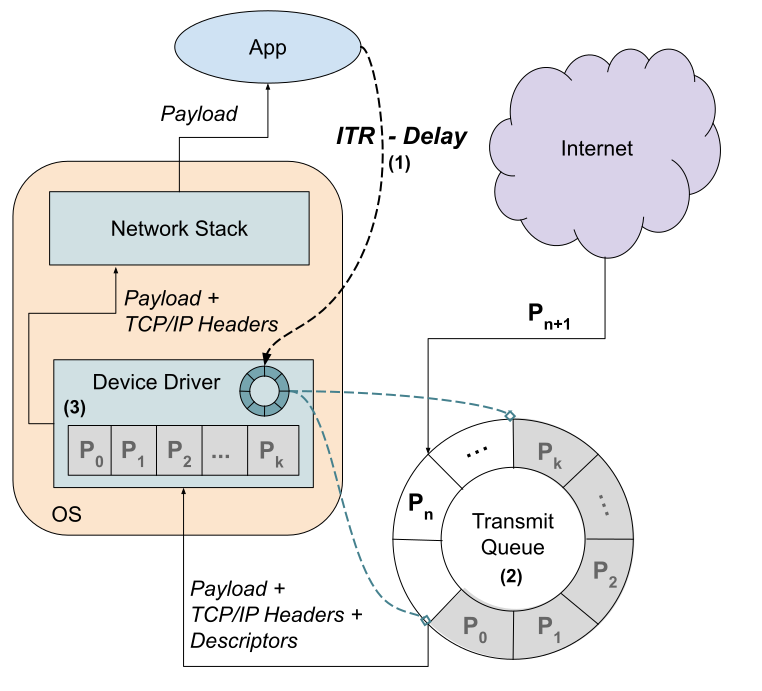
\includegraphics[width=7.7cm]{itr_figure.png}
\caption{As interrupt delay (1) is increased, the receive queue (2) buffers
more incoming packets as the NIC cannot fire new interrupts until the delay
value has been reached. Once the interrupt is fired, Linux's NAPI polling
mechanism kicks in and starts pulling in new packets (3) to be processed until
it either reaches its current work budget (calculated using existing jiffies)
or until there is no more data to be processed.}
  \label{fig:itr_figure}
\end{figure}

\subsection{Hardware Tuning Parameters}
Below, we discuss the three hardware parameters that are tuned statically in
this work:
\label{sec:knobs}
\begin{itemize}
\item \textbf{interrupt-delay}: Most modern NICs have a hardware feature to
control per receive interrupt rates.
The Intel 82599 datasheet~\cite{82599} defines a time-based interrupt
throttling mechanism which controls the time delay between packet reception and
the firing of an interrupt on the receiving core.
Its value can be set from a range between \texttt{0} and \texttt{1024}
$\micro$s in increments of \texttt{2} $\micro$s.
Figure~\ref{fig:itr_figure} illustrates the interaction of interrupt delay
values with the rest of systems software.
The effect of setting a higher interrupt delay results in potential buffering
of receive packets, thereby increasing packet processing efficiency at a
potential cost to response time.

Linux's network device driver uses a dynamic algorithm that seeks to tune the
interrupt delay value such that it better reflects the current workload.
It achieves this by using data received from the previous interrupt about
packet counts and bytes per packet.
These values are then used to classify the current state of the workload (ex:
latency driven vs. bulk compute) and tune the interrupt delay accordingly based
off pre-computed theoretical maximum wire speeds.
%received from the last interrupt and classifies them broadly into a set of
ranges that are pre-computed based off theoretical maximum wire speeds.
%This delay tuning is applied upon the next interrupt occurrence.
It is possible to disable this dynamic algorithm through the flip of a bit
inside the device driver. After flipping this bit, \textit{ethtool} can then be
used to set new interrupt delay values to statically fire at a fixed rate.
In our experiments, we take advantage of this ability by setting interrupt
delay values statically for different applications.
%device driver [REF] updates the interrupt delay value dynamically after every
packet receive to a value based on the current traffic pattern. This value can
also be fixed to a static value which results in interrupts being fired every X
microseconds where X is a configurable value.


%To demonstrate its behavior, we instrumented a simple logging tool into the
IXGBE device driver.
%Figure~\ref{fig:itr_delays} shows a small snapshot of its values while running
a Memcached workload.
%Each marker represents a new \textit{ITR-Delay} value.
%In its current implementation, it can only seek values between the range of 2
to 126 microseconds.
%The reason for this is that it was never designed towards a use case of
aggressively delaying packet receive interrupts to take advantage of energy
proportionality under stringent SLAs, which can potentially result in setting
\textit{ITR-Delay} values in the hundreds of microseconds.

%It is also possible to disable this dynamic algorithm through the flip of a
bit inside the device driver.
%This requires a rebuild of the driver module as it was not a configurable
parameter.
%After flipping this bit, we can use Linux's \textit{ethtool} to set new
interrupt delay values statically to fire every X microseconds, where X is a
configurable value.


\item \textbf{RAPL}: Running Average Power Limit (RAPL)~\cite{intel_rapl} is a
power limiting feature on Intel processors.
In our experiments, we use the RAPL model segment registers (MSR) registers to
set explicit power limits up to a default max of \texttt{135} Watts (\watt) in
a single package on the processor. The processor used in our experiments
contain two packages. When applying power limits, care must be taken to ensure
there is a minimum RAPL value such that an application's continued execution
can be sustained in this limited power budget.
%Applications often depend on hardware components that in turn rely on a
minimum power supply to continue running.
%Hence, when considering energy efficient compute, calculating minimum RAPL
values that would sustain the execution of a particular workload becomes
important.
From some initial experiments, we found that our class of applications
continued to execute correctly at a minimum RAPL limiting of around \texttt{55}
\watt. RAPL also provides the MSR\_PKG\_ENERGY\_STATUS register which allows
software to query the energy usage (Joules) of a specific package with a
minimum sample time of 1 milliseconds.
This is the main method with which our per-application energy consumption
results are gathered.

\item \textbf{DVFS}: Intel power states (p-states) is another energy saving
feature on Intel processors.
It allows users to set specific p-states for individual cores.
A p-state is a combination of the clock frequency and voltage that a core is
operating on. Typically,  p-states are set dynamically according to current
processor load by a policy governor in Linux called Dynamic Voltage Frequency
Scaling (DVFS). DVFS can be disabled, thereby enabling setting static p-state
values by writing to the IA32\_PERF\_CTL register~\cite{intel_msr}.
%A p-state is the combination of a core's clock frequency and its voltage at
some ratio, however, it is also unclear how it translates to real processor
frequency.
%Normally, p-states are set dynamically according to current processor load by
a policy governor in Linux called Dynamic Voltage Frequency Scaling (DVFS).
%In addition, DVFS can also be disabled which enables a user to set specific
p-state values by writing to the IA32\_PERF\_CTL register~\cite{intel_msr}.
From reading MSR\_PERF\_STATUS register~\cite{intel_msr}, we found the range of
DVFS values that a default Linux sets its processor into starts at a minimum
value of \texttt{0xC00} and up to a maximum of \texttt{0x1D00}. We use this
range in our study to tune processor p-states as another hardware knob.
\end{itemize}

\subsection{Per-interrupt Log Collection}
\label{sec:log_collect}
In order to better understand the interactions of interrupt-delay, DVFS, and
RAPL with a server that is under some load, we instrument \textit{fine-grained
per-interrupt} log collection in both Linux and library OS's network device
driver.
We collect the following information for every interrupt fired: received and
transmitted bytes, received and transmitted descriptors, and the current
timestamp (via \texttt{rdtsc} instruction).
In addition, we instrument per-core performance monitoring counters (PMCs) to
collect a set of hardware statistics after every millisecond of elapsed time:
instructions, cycles, reference cycles, last-level cache misses, and energy
used (using the MSR\_PKG\_ENERGY\_STATUS register).
This set of statistics helps us to both take a detailed look at the per-core
behavior and acquire a global perspective on overall resource usage when
hardware is tuned in different ways.
%While this data provides a breadth of directions to reason about the results
below, we discovered that it can be helpful to focus on subsets of data points
for different workloads.
We ensure that the logging mechanism adds minimal overhead to application
performance by using non-temporal store instructions to store the collected
statistics into an in-memory array.
%We found that using non-temporal store instructions had more of an impact on
the performance of EbbRT versus that of Linux.
%We believe that this could be due to the fact that EbbRT was built to be an
efficient library OS and hence its performance is more observably affected by
additional logging.
%\subsubsection{Measurements}
%\label{sec:measures}
%\begin{itemize}
%       \item Throughput and Latency: Throughput is defined to be the
time-average of total data transferred. It is measured in units of
[bytes/second].
%         Latency is a measure of the delay between a request and the
corresponding response. It is measured in [seconds]. Due to the stochastic
nature of latency, we follow the convention of measuring the 99th percentile of
the latency distribution for multiple requests.
%Depending on the workload, either throughput or latency is a direct measure of
network %performance.
         %[Any notes about exact measurement process?]
       %\item Energy and Power
    %     [Note about Joule counter]
         
     %  \item Instructions, Cycles, Cache-Misses
	%\item Device Driver Statistics
	%\item Sleep States
%\end{itemize}


\section{Experimental Setup}
\label{sec:exp_setup}
\subsection{Hardware}
Our experimental cluster consists of a total of 7 nodes with a mix of 16 core
Intel(R) Xeon(R) CPU E5-2690 @ 2.90GHz and 12 core Intel(R) Xeon(R) CPU
E5-2630L v2 @ 2.40GHz processors and NICs with a mix of Solarflare
Communications SFC9120 10G Ethernet Controller and Intel Corporation 82599ES
10-Gigabit SFI/SFP+.
The nodes have a mix of 126 GB and 250 GB RAM configurations.
The node used to boot into baremetal library OS and Linux contains a 16 core
Intel(R) Xeon(R) CPU E5-2690 @ 2.90GHz, with 125 GB of RAM and an Intel
Corporation 82599ES 10-Gigabit SFI/SFP+ NIC.
We ensured that the processor for both Linux and the library OS was setup as
similarly as possible by carefully configuring both IA-32 Architectural MSRs
and processor specific MSRs (Table 35-2 and 35-18 in Intel's system
programmer's manual~\cite{intel_msr}).

\subsection{Linux}
In order to ensure a fair comparison between an application running in a single
purpose library OS versus a general purpose OS, we create a set of Linux
appliances for each of the applications (see Section~\ref{sec:apps}) we intend
to run.
Their base OS is Debian 10.4 and we use a custom compiled 5.5.17 kernel built
using a modified configuration file built for performance following suggestions
from previous work studied Linux core operation
costs~\cite{10.1145/3341301.3359640}.

These appliances are specially constructed to run a RAM-based filesystem and
contain only a small set of system libraries and kernel modules required to run
their constituent applications. In order to minimize system noise, we disable
hyperthreads and Turbo Boost features on all  processors and pin all
applications to physical cores in order to reduce potential background noise.
In addition, ~\textit{irqbalance} is disabled and packet receive interrupts are
affinitized to their respective cores.

%Describe details of configurations considered and various policies and
mechanisms we know our workloads interact with.  Eg.  device driver, itr, napi,
idle sleep states, etc. Also discuss what app software used.

\subsection{Library OS}
We ported an existing library OS written in C++ to baremetal by writing a
network device driver for the Intel 82599 NIC. The device driver totals over
3000 lines of code and interfaces with its multicore TCP/IP network stack.

Our library OS's NIC driver inherently does not have a dynamic policy for
updating interrupt-delay values, this is due to the fact that Linux's dynamic
interrupt-delay policy implementation relying on particular assumptions about
jiffies and NAPI polling budgets which the library OS does not.

As our library OS follows an event-driven model, whereby on each core, an
interrupt is fired after every static period of time to check a list for new
events to process; we implement a simple idling algorithm in this event loop by
adding \texttt{monitor} and \texttt{mwait} instructions in order to recommend
an idling core to go directly into the deepest sleep state prior to the
execution of a \texttt{halt} instruction. The sleep state value is inferred
from the \texttt{intel\_idle} function in Linux for our specific processor. The
library OS's idling policy is more simplistic compared to Linux, which consist
of multi-level sleep states dependent on the current system load.

%We were careful to ensure that both EbbRT and Linux were configured similarly
in terms of NIC features: receive-side coalescing (RSC) disabled, direct-cache
injection (DCA) disabled, receive-side scaling (RSS) enabled to distribute
packets for multi-core processing, hardware checksum offloading enabled. We
also ensured the same values for parameters such as number of NIC transmit,
receive descriptors and write-back thresholds for packet transmissions.

%Describe relevant background focusing on device driver, itr, and idle
behavior. Also discuss benchmark app software.


%\subsubsection{Tuning Methodology}


\subsection{Applications}
\label{sec:apps}
In this study, we use the following set of applications in order to cover a
range of network workloads.
\begin{itemize}
\item \textbf{Netpipe}~\cite{snell1996netpipe} involves sending messages of the
same size between two systems for a fixed number of iterations in a single
connection. Both the client and the server are single-threaded. In both
systems, the 10 GB link is close to saturation after a message of size over 700
KB. We fix the iteration count at 5000 and show results for a range of message
sizes.

\item \textbf{Nodejs}~\cite{nodejs} consists of of a single client thread and a
single server thread with a single connection between them. The server is
running a simple server written for nodejs using its builtin \texttt{http}
module that responds to each GET request with small static messages of size 148
bytes. A single client running the wrk~\cite{wrk} benchmark is used to place a
load on the nodejs server for a total of 30 seconds.
%In contrast to netpipe, the workload is not fixed and performance is measured
in requests-per-second once the benchmark has finished running. Further, a
nodejs web server is computationally heavier than netpipe.

\item \textbf{Memcached}~\cite{mcd} is a multi-threaded application that runs
on all 16 cores of our server node.
The SLA objective in this application is to maintain a tail latency defined by
99\% of requests being processed in under 500 $\micro$s.
A client node running mutilate~\cite{mutilate} with no additional network load
is the main driver for controlling and monitoring the experiment.
It has two responsibilities: (1) it coordinates with five other mutilate agent
nodes in order to generate requests to the server and (2) measures tail latency
of all requests made.
One of the five agent nodes is a 12-core machine while the rest are 16-core
machines. Each core creates 16 connections, for a total of 1216 connections
amongst 5 nodes. This setup is able to saturate the single 16 core server.
Mutilate is configured to pipeline up to four connections to further increase
its request rate.
We run a representative load from Facebook~\cite{workloadanalysisfacebook}
(ETC) which represents the highest capacity deployment. It uses 20 - 70 byte
keys and 1 byte to 1 KB values and contains 75\% GET requests.
	
%\item \textbf{Memcached-silo}~\cite{mcdsilo} is an addition on top of the
normal memcached protocol used to reflect a more complex workload which
includes a combination of latency sensitive network traffic and compute and
memory intensive TPC-C style transaction processing.
%We ported memcached-silo, that was developed by previous work done on building
scalable $\micro$s-scale in-memory compute servers~\cite{zygos}, to the library
OS.
%The configuration and SLA of memcached-silo follows from that of memcached
(listed above). Given its computationally heavier nature, we only needed two
16-core server nodes at 16 connections per core to saturate our memcached-silo
server.
\end{itemize}

\subsection{Hardware Tuning Methodology}
\label{sec:hw_tuning}
We statically set interrupt-delay, DVFS, and RAPL values on the server node of
every application and collect per-interrupt log statistics on the same machine;
the range of values with which we vary these hardware parameters are listed in
Section~\ref{sec:knobs}.
It should be noted that for each application, we further reduce the sets of
values explored based on small experiments done a priori. Some of these are due
to ensuring that (1) increasing interrupt-delay and lowering DVFS processor
frequency does not bring about SLA violations for the memcached applications,
(2) lowering RAPL power limits does not cause the application and/or overall
system to crash, and (3) hardware configuration values encompass a wide range
and can be applied towards a specific workload, and (4) allows us to gather all
the results in a timely manner.

Below, we list the additional details of hardware tuning on a per-application
basis:
     
\begin{itemize}
\item \textbf{Netpipe}: Four representative message sizes of 64B, 8KB, 64KB,
and 512KB with a fixed round trip of 5000 iterations are selected. In addition,
as netpipe consists of the same binary running both as a client and a server,
we configured interrupt-delay to be the same in both client and server nodes.
For each message size and hardware configuration, we run the experiment 10
times to ensure statistical stability.
    
\item \textbf{Nodejs}: The wrk~\cite{wrk} benchmark is used to place a load on
the nodejs server for 30 seconds. We only apply hardware configuration on the
server and rerun the experiment 10 times as well.
    
\item \textbf{Memcached}: Mutilate is used to generate three different
requests-per-second (QPS) rates of 200K, 400K and 600K for a fixed period of 30
seconds each. For each QPS rate, we run it across the three systems 5 times for
statistical stability.
    
%\item \textbf{Memcached-silo}: Lower QPS rates of 50K, 100K, and 200K are
targeted here due to its increased computation load per request. Similarly, per
QPS rate is run on all three systems 5 times each.
\end{itemize}



%     \item The experiments are run for various ITR, DVFS, and RAPL settings.
In the single threaded workloads, RAPL was fixed at the linux default value of
135 \watt since we found it had minimal impact compared to ITR and DVFS on
total time and total energy in both Linux and EbbRT. We hypothesize this is
because RAPL power limiting is applied to an entire CPU package, therefore the
power used in running a single threaded application was not heavy enough to
warrant the power limiting features to come into play.
%     \item Each experiment can be described uniquely by the configuration
tuple - (OS, MSG, ITR, DVFS).
%     \item Each configuration was run 5-10 times to measure statistical
stability.
%     \item When the OS is Linux, we use three distinct configurations:
%        \begin{itemize}
%            \item Default - Both ITR and DVFS are changed according to the
default Linux policy.
    
%            \item Tuned: DVFS -  ITR varies according to the default Linux
policy while DVFS is fixed to a constant. The value reported in this column
corresponds to the configuration (searched across DVFS values) that results in
the smallest EDP. The smallest EDP and the corresponding Throughput for the
same configuration are reported.
            
%            \item Tuned: DVFS + ITR + RAPL are fixed to constant values. As
before, the smallest EDP (searched across ITR, DVFS, RAPL) is reported along
with the corresponding performance value.
            
%        \end{itemize}
%    \item Since EbbRT does not implement dynamic policies for either ITR or
DVFS. we use two distinct configurations:
%        \begin{itemize}
%            \item BaseLine - This column measures EDP and Throughput for the
best Linux configuration found by tuning both ITR and DVFS. This is a direct
comparison of the two OS structures.
            
%            \item Tuned - This column reports the smallest EDP (searched
across ITR and DVFS) and the corresponding Throughput value.
            
 %       \end{itemize}

%\subsection{NetPipe}
%\label{sec:exp_app:netpipe}
%\begin{itemize}
%    \item We run the experiment with four message sizes (MSG) - 64B, 8KB,
64KB, and 512KB on each of Linux and EbbRT. Each experiment involves
transmitting packets of fixed size for 5000 round trips between two machines
running the same operating system (OS). The total time taken (T) and the total
energy consumed (E) are measured.

%    \item For each unique configuration, we measure the average EDP
(Energy*Time) and average Throughput (MSG * 5000 / Time). The averages and
standard deviations are across the runs for each configuration.

%    \item Table \ref{tab:netpipe_linux} lists both the EDP and Throughput
values
        
%    \item Table \ref{tab:netpipe_ebbrt} lists both the EDP and Throughput
values for the following cases when the OS is EbbRT  (columns 5 and 6 of table
\ref{netpipe_linux}).

%\end{itemize}

%\subsection{NodeJS}
%\label{sec:exp_app:nodejs}
%\begin{enumerate}
%\item A simple web server written for nodejs using its builtin http module
that responds to each GET request with small static messages totaling 148
bytes, pinned to one core. A single client running wrk~\cite{wrk} benchmark to
place a load for 30 seconds. Throughput is measured in requests/sec achieved
once the benchmark is finished.
%\end{enumerate}

%\subsection{Memcached}
%\label{sec:exp_app:mcd}
%\begin{enumerate}
%\item 16 core memcached server=
%\item Given a static configuration listed above, we use \textit{mutilate} to
generate loads at different request per second (RPS) rates, each for a constant
period of time while collecting additional system metrics. In Linux,
\textit{perf} is used to gather these metrics at a per second timeslice since
the MSR\_PKG\_ENERGY\_STATUS for reporting CPU power usage has a limited wrap
around time. EbbRT is able to collect the same metrics as Linux as it contains
a inbuilt ~\textit{Perf} class which reads directly from Intel's PMC registers
and a ~\textit{Rapl} class which reads from Intel's RAPL registers. In EbbRT,
an event is triggered to fire every second in order to log the corresponding
data.
%\end{enumerate}


\label{sec:related}

% Table in google docs
% Cloud service focus -- extends the notion of slowing down to include delaying of request detection using interrupt delaying -- versus only considering power management mechanisms.

% OS focused analysis: We focus on understanding how the OS's structure impacts and interacts with the net performance realized and energy consumed.  
% (Gernot work examines the knobs but not the impact of changing the OS)

% General model that frames software behavior that can be adapt as hardware tradeoffs change 

% We use existing interrupt delay feature to delay packet detection when using interrupts.

% Exhaustively document the behaviour of real software

% Closed loop and open loop model 

% we ask questions regarding OS role in energy proportional computation
The questions that our investigation sparked fall within a wider space of research on the impact of OS design and hardware and software policies on the incessant goal of energy proportional computation in datacenters~\cite{energyproportion, warehouse-power, 268014}. Much of this research stems from the challenges of improving the performance of network-bound datacenter workloads like MapReduce~\cite{large-scale-mapreduce} and in-memory key-value stores~\cite{mica, zygos} while keeping energy consumption at bay. These challenges can be attributed to
the complex diurnal trends that are characteristic of datacenter-level utilization, whereby idle time is common and must be optimized for~\cite{hotpower2008, powernap, napsac} while simultaneously maintaining the ability to support high-utilization peaks and strict latency constraints ~\cite{Dynamo, SmoothOperator, oldi-pegasus, adrenaline, rubik, eurosys14, zygos, peafowl, 7425206, 10.1145/2830772.2830779, dreamweaver, dynsleep, udpm}. Our work examines both in-memory key-value stores and its modified version with a heavier processing component as well as closed loop applications. Our incessant goal was not to design another dynamic policy but to gain better insight into the systemic impacts of performance and energy when slowing down these web-centric workloads using two mechanisms together.

There is a wide range of work that targets energy proportionality with a focus on designing OS policies and mechanisms for power management. Most of this work presents hardware level optimizations that manipulate processor speed mechanisms such as DVFS ~\cite{10.5555/2523721.2523732,10.1145/381677.381702,cpufreq_governor,4273098,packandcap,10.1109/MICRO.2006.8,1598114,10.1145/1629911.1629926,4658633,4343825,10.1109/IGCC.2011.6008552,10.1145/1241601.1241609, slowdownorsleep,4228267, mootaz}, processor power limiting mechanisms such as RAPL~\cite{intel_rapl, heracles, SmoothOperator,oldi-pegasus, Dynamo,PerAppPower,powercap}, and idle power states~\cite{cpuidle_policy,peafowl, udpm,6983037,dreamweaver, pacingtoidle} (c-states) by applying feedback control mechanisms and relying on activity models. The authors of ~\cite{heracles} and ~\cite{PerAppPower} go a step further, exploring and characterizing the interference of co-located latency-critical versus best-effort tasks and high versus low CPU demand tasks when subject to energy tuning via DVFS and RAPL. In doing so, they highlight limitations in using hardware features alone for power management. Similarly, the authors of ~\cite{hotpower2008, 7349225} identify a need to step away from relying entirely on hardware solutions and focusing instead on software optimizations, such as VM migration controllers for power management of an ensemble of nodes. Previous works have advocated for full-system and hardware optimizations for energy~\cite{slowdownorsleep,powernap}, our work builds on their observations and assert that the OS itself plays a big role as well. 

These previous research efforts present significant energy savings from well designed dynamic policies and carefully chosen static configurations, however, we are driven to explore the space beyond current findings with a focus on unveiling the role of the OS in exploiting activity and idleness and also by introducing interrupt delay as an additional knob in this exploration. We find that this exploration is timely given the range of work on optimizing OS paths for performance, from NIC driver mechanisms~\cite{flexnic, affinityaccept, network-latency} to the network stack~\cite{mtcp, sandstorm, network-latency} and the dataplane~\cite{222583, arrakis, EbbRT, shenango, zygos, ix}. Our work was also influenced by previous work in energy efficiency by slowing down both the networking and processor: $\mu$DPM~\cite{udpm} is a application-level policy for memcached to delay request processing and maximize idle periods where deep sleep states can then be utilized, in ~\cite{10.5555/2338816.2338822} the authors combined bandwidth limiting in Cray clusters and scaling processor frequency to reduce energy use of HPC applications. In contrast to $\mu$DPM, we use a hardware register on the NIC to induce interrupt delays and this mechanism can be commonly found in commercial NICs. Lastly, in contrast to all of the previous works, we are the first to conduct such an in-depth study with a bare-metal specialized OS.

%Our work was also motivated by prior research in designing policies using DVFS, request delaying, and c-states to save energy.

%Slowing down Request delaying along with 

%c-states: idle power states
% Dynamo~\cite{Dynamo}, Pegasus~\cite{oldi-pegasus}, Adrenaline~\cite{adrenaline}, and Rubik~\cite{rubik} use the above hardware features to tune power-draw across various applications.

%notable limitations of p-states and c-states
%\cite{oldi-study} presents some of the limitations of restricting power management to hardware tuning, and \cite{powercap} compares the merits and limitations of different hardware and software power management techniques. These results led us to study the power management of OS-centric and application-centric tasks during idle and active utilization and the time spent in between. The system is often not idle but only slightly busy, yet system sleep states present a challenge in resuming high activity in response to sudden bursts while system polling maintains support for high activity but degrades energy efficiency. In response to this, the authors of \cite{oldi-pegasus} define an iso-latency policy that aims to maintain energy proportionality at variable, dynamically shifting activity levels via OS-level optimizations.







%Hence we consider an OS-level study with an interrupt-centric experimental methodology for exploring idleness, activity, and the dynamic lapses in between.
%INJECT MOTIVATION




% %INJECT CONTRIBUTION
% This work
% started with a motivation to study the impact
% of a NIC hardware parameter, ITR-delay,
% alongside well studied DVFS and RAPL parameters~\cite{rapl2015, rapl2018},
% on energy consumption
% of a baremetal libOS in contrast to general purpose Linux.
% We wished to quantify the benefits that a libOS,
% specialized and optimized for network-bound work,
% can have on energy proportionality.
% Our efforts concluded with several interesting findings,
% one of which is the realization of a potential hybrid solution
% for manipulating system idle time in our libOS,
% whereby the OS switches from interrupt-driven
% %(which assumes clear separation of idle and busy activity)
% to polling-driven execution
% %(which takes a more intermediary position)
% under particular hardware energy configurations.
% %add result: less interrupts? more energy saving? better performance?
% These findings would not have come to light
% were it not for the structure of the libOS
% and its particular event-driven execution model~\cite{seda, unikernels}.
% %ebbrt
% They help us assert that we cannot disregard the OS
% as a constituent contributer to application performance and overall cycles-per-instruction (CPI).

%			
%when limitations are reached,
%OS level software optimizations
%--> vm migration
%--> nic controllers
%--> network stacks (libOSes and appliances)
%--> dataplane separation from control plane (ix, arrakis)


%INJECT MOTIVATION
%now the impact of OS path lengths and low level OS behavior becomes primary target for research
%--> hence our motivation for this detailed study of libOS performance vs general purpose linux performance
%--> particularly with emphasis on network and data bound performance

 


\section{Results}
\label{sec:results}

For every application used in our experiments, we label results from the  three \textit{systems} as:
%In our results below, we present data points for three main systems in each application workload:
\begin{itemize}
    \item \textbf{Linux Default} refers to normal Linux where both the interrupt-delay and DVFS values are set by their dynamic policy.
    \item \textbf{Linux Tuned} and \textbf{Library OS Tuned} refer to Linux and the libOS where the hardware parameters are statically tuned such that EPP is minimized.
\end{itemize}

\subsection{Netpipe}
\label{sec:results:netpipe}
%By tuning ITRDVFS, we achieve a 4x decrease in total time spent on this workload, though that comes at a cost of higher energy consumption rate in Linux tuned.

%This figure also provides context for the interactions that occur between the message size, the protocol stack and the bytes on the wire as message size change. At a large 512 KB message, the network becomes the bottleneck and all three systems start converging at peak throughput, as a larger faction of time is spent on the wire and the system' idle time proportionally increases.  At small to medium sizes more time, per-round trip, is spent in the system code; device driver and protocol processing, thus the load on system's software is proportionally higher.

%At larger message sizes the systems ability to detect and exploit large idle times will be exposed and at small message sizes the systems software's efficiency will be highlighted.  Medium messages sizes will expose a mixture of the systems ability to detect and exploit idle opportunities while also exposing its packet processing efficiency. The less time spent packet processing the greater the opportunity to idle.   

%, thereby illustrating the latency and throughput trade-offs in this application.

%TODO YA
%This figure has the potential to provide context of the different interactions that occur between the workload, protocol stack, and bytes on the wire as message size changes, which illustrates the latency and throughput trade-offs in this application.
%We hypothesize that this result is mainly due to the inefficiencies of the dynamic itr-delay algorithm to adapt to a simple ping-pong workload where a simple static itr-delay value set to a message specific size can result in improved packet processing efficiency. \textbf{as message size changes the workload changes with respective to the protocol stack and bytes on the wire, system tradeoff between latency and throughput changes as size changes}

%% \begin{figure}
%% 	\includegraphics[width=\columnwidth]{asplos2021_figures/netpipe_edp_8192.png}
%% 	\caption{Plot for a fixed message of 8 KB where EDP is minimized.}
%% 	\label{fig:netpipe8192edp}
%% \end{figure}	
%% \begin{figure}
%% 	\includegraphics[width=\columnwidth]{asplos2021_figures/netpipe_combined_barplot_8192.png}
%% 	\caption{Raw data collected from logs for 1 sample run of message size 8 KB normalized to Linux default.}
%% 	\label{fig:netpipe8192bar}
%% \end{figure}

\begin{figure}[t]
  \includegraphics[width=\columnwidth]{osdi_figures/netpipe_tput.pdf}
  \caption{Throughput results across message sizes when tuned for performance.}
  \label{fig:netpipe_tput}
\end{figure}

Figure~\ref{fig:netpipe_tput} illustrates results from a pure throughput perspective across four message sizes (64B up to 512 KB).
By tuning the ITR to a fixed value, we are able to a find a specific hardware configuration for each message size that optimizes overall throughput.
Linux tuned results in a 1.5X to 2X improvement in throughput across message sizes, the libOS further improves the performance by a factor of 1.6X to 3X as compared to Linux. Figure~\ref{fig:netpipe_tput} also shows that as payload size increase, the network becomes the bottleneck and all three systems start converging at peak throughput; this implies that as a larger faction of time is spent on the wire, potentially increasing each systems' idling time. At small to medium payload sizes, there is more of a mix between packet transmission time and time spent in the system code, device driver, and protocol processing.

\subsubsection{General Observations}
From the datapoints listed in Table~\ref{table:eppsum}, Linux tuned outperforms default Linux across all four message sizes in EPP by up to 60\%, further, the LibOS outperforms Linux default across all four message sizes by up to 80\%. We find that in all cases, this is achieved by reducing both time and energy to complete the offered load. We found RAPL to play a minimal role in power tuning for this application given it is not a processor nor memory intensive workload and runs on a single core. In order to observe general trends of hardware tuning effects on Linux and the libOS, we examined the data from a set of low EPP configurations. We found that at smaller message sizes (64 B, 8 KB), ITR plays a pivotal role in reducing EPP given that vast majority of ITR values were less than 10 \micro s, however, there was wide variations in DVFS values for us to make a statement about its usefulness at low message sizes, we suspect the system is largely too lightly loaded for it to play a role. At a message size of 64 KB, the ITR values have largely moved to the 8 - 30 \micro s range, and at 512 KB to the 26 - 38 \micro s range - this is due to packet transmission becoming a larger bottleneck, the larger ITRs used by both Linux tuned and libOS imply a form of artificial packet coalescing is being induced. At these larger message sizes, DVFS plays a more profound role as we see values between \texttt{0xc00 - 0x1500} being consistently applied by Linux tuned and \texttt{0xc00 - 0x1000} being used by the libOS. In addition, the libOS is able to set its DVFS at a value due to its smaller overall codebase, we find that across all message sizes, the instruction usage of libOS is 43\% - 80\% less than Linux and suffered 71\% - 97\% less last-level cache misses. These instruction level efficiences enable the libOS to support the workload while drastically lowering its energy usage through reduced processor frequency; this is also supported by the fact that the libOS's energy usage fell by a greater percentage than time used in the larger message sizes.

\begin{figure}[t]
  \includegraphics[width=\columnwidth]{osdi_figures/netpipe_524288_epp.pdf}
  \caption{Plot for a fixed message of 512 KB where EPP is minimized.}
  \label{fig:netpipe524288epp}
\end{figure}

\begin{figure*}[htb]
\centering	
\begin{minipage}[t]{0.45\textwidth}
\includegraphics[width=\textwidth]{osdi_figures/netpipe_524288_barplot.pdf}
	\caption{Raw data collected from logs for 1 sample run of message size 512 KB normalized to Linux default.}
	\label{fig:netpipe524288barplot}
\end{minipage}
\begin{minipage}[t]{0.45\textwidth}
	\includegraphics[width=\columnwidth]{osdi_figures/netpipe_524288_nonidle_timeline.png}
	\caption{Per-interrupt non-idle ratio for 512 KB message.}
	\label{fig:netpipe524288nonidle}
\end{minipage}
\begin{minipage}[t]{0.45\textwidth}
	\includegraphics[width=\textwidth]{osdi_figures/netpipe_524288_joule_timeline.png}
	\caption{Per-interrupt joules consumed for 512 KB message.}
	\label{fig:netpipe524288joule}
\end{minipage}
\end{figure*}


\subsubsection{512 KB Analysis}
Figure~\ref{fig:netpipe524288epp} shows the joules consumed as a function of time across the length of the workload that sends fixed-size 512KB messages over 5000 round-trips. The line is generated from the detailed per-interrupt log data, the points illustrated are a sub-sampling to improve legibility.  
The slope in this figure is representative of the rate of energy consumption for each system.
Through hardware tuning, Linux achieves 25\% savings in EPP and the libOS achieves 37\% savings, moreover, the rate of energy consumption has also been lowered.

%Figure~\ref{fig:netpipe8192edp} shows the EDP of running our workloads across the three systems upon tuning the aforementioned hardware knobs  towards lower EDP.

%%This figure shows the joules consumed as a function of time across the length of the workload that sends fixed-size 8KB messages over 5000 netpipe round-trips. The line is generate%%d from the detailed per interrupt log data, the points illustrated are a sub-sampling to improve legibility.
%The slope in this figure is representative of the rate of energy consumption for each system.

%By tuning interrupt-delay and DVFS, we achieve a 4x decrease in total time spent on this workload, though that comes at a cost of higher energy consumption rate in Linux tuned.

Figure~\ref{fig:netpipe524288barplot} shows some collected log data gathered from one sample run of this workload and are all normalized against Linux default. Note, the smaller data transmitted in libOS is due to its simpler TCP/IP stack where there are less options used in its TCP/IP header packets. We observe that while the static tuning of Linux and the libOS both reduced the workload in time and used less energy, the number of interrupts was actually 2X higher than default Linux. We attribute this high number of interrupts to be the statically set ITR delay value of 28 \micro s and 26 \micro s for Linux tuned and libOS respectively. This difference is illustrated in figure~\ref{fig:netpipe524288timediff}, where the time difference between every hardware interrupt is shown as function of time for the entire experiment - this figure shows a much wider range of time between interrupts for default Linux. It also shows that tuned Linux's time between every interrupt is roughly concentrated on the ITR delay value that was set, similar to the libOS, except the libOS also exhibits interrupts with wider differences between them. The implication of these diferences are dependent upon the system.

Figure~\ref{fig:netpipe524288nonidle} shows the percentage of time each system was non-idle every 1 ms (this is due to the sampling period we used in this study for reading PMC registers), the non-idle value is derived by taking the ratio between fixed reference cycle data, which measures un-halted core cycles, and the difference between timestamps. From this figure, we can see distinct behaviors between tuned Linux and the libOS where tuned Linux spent most of its time busy to finish the work fast while the libOS was able to both finish the work fast but also take advantage of idling opportunities. The result of this behavior is shown in figure~\ref{fig:netpipe524288joule}, where the two effects of hardware tuning causes the average energy consumption to be lower than Linux default - the 0 joules in figure~\ref{fig:netpipe524288joule} are due to the fact the joule register can only be sampled at a minimum time interval of 1 ms. The efficiency of the libOS and its ability to idle can be seen in figure~\ref{fig:netpipe524288barplot} where the libOS halted into \texttt{C7} sleep state 3X higher than Linux default and the fact the libOS' CPI is 40\% lower. It is also interesting to note tuning Linux resulted in a completely different behavior in terms of idling state where the tuned Linux concentrated all of its idling in the \texttt{C1} state. We hypothesize this is due to the frequent interrupts invoked by the static ITR delay affecting Linux's scheduler. Moreover, the wide range the libOS' time between interrupts could be explained by the high number of \texttt{C7} sleep states as a \texttt{C7} sleep state has exit latencies in the order of hundreds of microseconds while the \texttt{C1} sleep state's exit latency is 2 \micro s.Moreover, even though Linux tuned could not idle as efficiently as the libOS, both systems could set DVFS to a low value of \texttt{0xc00}. We believe this is due to the network heavy nature of NetPIPE when exchanging 512 KB messages, the benefit of this low DVFS value results in a greater percentage of energy savings than time savings for both tuned Linux and the libOS.

%Compared to default Linux, summing up the total number of times c-state was entered, we found tuned Linux idled 23\% less and the libOS idled 96\% less, however the nature of these sleep states counters do not specify 

%This points to greater aggregate workload efficiency coming from fixed lower interrupt delays, 8 $\micro$s and 6 $\micro$s respectively, than what the default algorithm chooses over the life time of the experiment.   This increase in interrupts in 
%tuning Linux results in a 15\% increase in the overall number of instructions executed, however, the temporal savings this translates to yields a significant improvement in energy used and the energy efficiency of the other metrics.  In some sense tuning allow the systems to race to halt to get the work done by  burning energy at a slightly greater rate but using it more efficiently.  

%In our library OS, the number of instructions per interrupt is lower despite a small increase in total interrupt count due to the smaller interrupt-delay value, it also uses dramatically fewer instruction. This results in a considerably higher Bytes transmitted per joule efficiency. A library OS has shorter path lengths due to its dedicated and simplified processing model, further, as application code is executed in the same privileged domain as the device and protocol code and runs in an integrated fashion with the receive interrupt handler. 


%the energy used to satisfy the same work decreases by 3x.
%This speaks to the instruction efficiency of tuning in relation to improving packet processing time.
%Moreover by tuning a library OS, we are able to both reduce instruction count and energy use while supporting the same workload. 

%% \begin{figure}
%% 	\includegraphics[width=\columnwidth]{asplos2021_figures/netpipe_timeline_joules.png}
%% 	\caption{Per interrupt measure of Joule collected for Netpipe 8KB.}
%% 	\label{fig:netpipe8K_joule_tsc}
%% \end{figure}

%Further packet processing efficiency can be seen in figure~\ref{fig:netpipe8K_joule_tsc}, where the per-interrupt number of joules consumed is shown.
%As joules can only be sampled at a minimum time interval of 1 ms, all three systems will exhibit instances in which the time between interrupts is less than 1 ms.
%This is accounted for in the graph by the bottom band of points that report 0 joule energy consumption. These points effectively visualize the temporal interrupt activity that contributes to the 1ms separated Joule readings.  At the scale plotted, it is a hard to compare the interrupt activity captured by the zero points, however, the interrupt bars of Figure~\ref{fig:netpipe8192bar} can be used to infer the relative difference in density of interrupts along the zero line.

%In default Linux, we see two distinct bands of joules consumed, a sparse band showing higher joule consumption, and a dense middle band showing lower joule consumption.
%A simple back-of-the-envelope calculation summing the joules and dividing by the total time gives us a measure of power at 17.29\watt.  This value is very close to the number we have measured when Linux and our library OS are completely idle, with no user applications launched, and they are able to use the deepest sleep state of the processor for the period that their idle behaviour can halt the processor.  

%It should be noted that an OS idling often involves some component of non-halted, time to conduct various  \textit{idle work} -- maintenance and background system work.  Furthermore,  despite being idle once there is application and network activity an OS may have more "idle work" that it must do and the nature of this work maybe stochastic in its costs (eg. uneven garbage collection work).  Despite halting the processor, the OS may use different and less aggressive sleep states given some algorithm it may have for predicting the value and penalty of the sleep states.  While this is true for Linux which is designed to run many applications over many different scenarios, the library OS we use adopts a simple fixed policy of always halting to the deepest sleep state.  

%With the above in mind, we observe fascinating phenomena when considering Figures~\ref{fig:netpipe8K_joule_tsc} and ~\ref{fig:netpipe8Knonidle}. Figure~\ref{fig:netpipe8Knonidle} is derived by taking the ratio between fixed reference cycle data point, which measures un-halted core cycles, and the measured diff between timestamps. 

%Linux default has a bi-modal behavior where it shows a slow steady rate of work that also idles efficiently (close to the best idle power consumption). Unfortunately this drags the total time well beyond what it could have achieved, in other words it neither raced-to-halt globally nor locally. Moreover, when it is doing work it is also more inefficient compared to Linux and the library OS tuned by using more Joules. However, while Linux tuned also managed to race-to-halt globally per interrupt, it was over 50\% busy, which suggests its algorithms averaging its power consumption between the idle consumption and the busy consumption. In contrast, the library OS's shorter path length and simple idle behaviour allow it to both race to halt globally and between interrupts. Thus the library OS is more effectively exploiting the IO nature of the workload to lower the energy consumption. 
%we observe when default Linux is servicing a packet.  
%This power number is exactly the per-package idle power number that we also measured from past experiments.
%This results tells us that the default Linux policy causes Linux it to spend more time idling (the middle band) than actually doing work (the highest band) and is therefore another contributing factor to its EDP. 

%In tuned Linux, there seems to be no idling time at all due to the use of an extremely fast interrupt-delay of 8 $\micro$s, which suggests the benefit of quick turn-around-time for this particular workload.
%Interestingly, while the library OS uses an even smaller interrupt-delay of 6 $\micro$s, it manages to both respond to packets quickly and take advantage of slack time to idle and conserve more energy.
%Moreover, the library OS's instruction efficiency allows it to tune processor frequency at a lower value than tuned Linux.
%The difference between the library OS's idle efficiency and that of tuned Linux is shown in  figure~\ref{fig:netpipe8Knonidle} which uses data from reference cycles collected.
%Reference cycles count the un-halted core cycles that are not affected by processor frequency tuning.
%Therefore, they can be used to infer potential energy savings from idling by observing its ratio with the timestamp counter.
%NOTE FOR YA
%linux is mostly idling
%linux tuned idles least
%lib os tuned idles more or simply executes less overall

%% \begin{figure}
%% 	\includegraphics[width=\columnwidth]{asplos2021_figures/netpipe_nonidle_8192.png}
%% 	\caption{Non-idle ratio for fixed message size at 8 KB}
%% 	\label{fig:netpipe8Knonidle}
%% \end{figure}

%Perhaps a potential benefit of the packet transmission behavior a library OS results in the ability to idle at a more efficient rate. In both systems, when there are no packets to be processed the processors are idling and will be put into some sleep state. These sleep states consists of different levels of energy savings by turning off various processor features.  This figure shows that while Linux default spends 20\% of its time processing and therefore 80\% of its time idling, potentially saving energy by going into sleep states, the increased overall processing time means the base idle cost is still a major contributor to overall energy usage. However we find that by using a library OS, it results in middle ground such that the shortened processing time and the simple packet transmission ability of its device driver results more idle time percentage as compared to Linux tuned. 

%\indent \textbf{summarize results from other message sizes}
%While our study includes detailed experiments for the netpipe workloads at other message sizes, however due to space concerns, we choose to focus on the 8K message size for detailed presentation as it allows one to observe a balance in how the systems behave with respect to busy and idle behavior.  With other message sizes the basic trade-offs remain but in different proportions: 1) at 64 byte messages tuning Linux to minimize EDP reduces the time and energy by 25\% and tuning the library OS by yields a 50\% reduction in time and energy compared to Linux default, 2) at 64KB message size 40\% reduction in time and energy for tuned Linux and 60\% for library OS, and at 512 KB message size 5\% and 10\% respectively.


\subsection{NodeJS}
\label{sec:results:nodejs}
%In the next application, a benchmark sends a constant rate of http requests to a single threaded webserver deployed using the http module running inside a nodejs process. In contrast to the simplified round trip behavior of netpipe, this webserver incurs a heavier processing burden.  Across 
% Even in this regime, tuning hardware knobs matters in both Linux and the library OS
%\begin{table}[]
%\begin{tabular}{| c | c | c | c | c | c |}
%\hline
%           & \multicolumn{4}{c |}{Latency ($\micro$s)} &   \\ \hline
%           & 50\% & 75\% & 90\% & 99\% &  Requests\\ \hline
%\begin{tabular}{@{}c@{}}Linux \\ Default\end{tabular}    & 81   & 82   & 85   & 91   & 365758         \\ \hline
%\begin{tabular}{@{}c@{}}Linux \\ Tuned\end{tabular}    & 74   & 76   & 79   & 85   & 394704         \\ \hline
%\begin{tabular}{@{}c@{}}Library OS\\ Tuned\end{tabular} & 59   & 60   & 61   & 68   & 491765         \\ \hline
%\end{tabular}
%\caption{NodeJS Performance Data}
%\label{tab:nodejs}
%\end{table}
%% across the latencies, variance is mostly similar, 99% tail latency is this, and translates to this throughput

%Table~\ref{tab:nodejs} illustrates the base performance of running a webserver in nodejs. Linux tuned is able to achieve 8\% higher requests than default just by disabling its default DVFS and itr-delay policy and selecting a set of static values that maximizes its performance, while the library OS improves performance by 35\%. With
% for computational work you do have to do, if 
\begin{figure}[t]
	\includegraphics[width=\columnwidth]{osdi_figures/nodejs_edp.pdf}
	\caption{NodeJS EPP plot across three systems}
	\label{fig:nodejs_epp}
\end{figure}
\begin{figure}[t]
	\includegraphics[width=\columnwidth]{osdi_figures/nodejs_barplot.pdf}
	\caption{Collected datapoints of NodeJS across three systems normalized to Linux Default}
	\label{fig:nodejs_bar}
\end{figure}
\begin{figure}[t]
	\includegraphics[width=\columnwidth]{osdi_figures/nodejs_instructions_timeline.png}
	\caption{NodeJS: Per interrupt instruction count.}
	\label{fig:nodejs_instruction}
\end{figure}

\subsubsection{General Observations}
In contrast to NetPIPE, with the move to a processing heavier workload, we found the top minimum EPP points all used ITR delay values of 2 and 4 \micro s for both tuned Linux and the libOS. The efficiency of the libOS over Linux is more dramatic here as the minimum EPP for Linux tuned all required setting DVFS at the higher frequencies (0x1b00-0x1d00), whereas the libOS is still able to lower its processor frequency (0x1900-0x1b00) to conserve additional energy. For the minimum EPP of Linux tuned, DVFS was set at the highest setting along with RAPL while ITR delay was set at lowest value of 2 \micro s. Given these settings, tuning Linux was able to lower its EPP over Linux default by 16\%, the libOS was able to lower its EPP of Linux default by 55\%. In both tuned settings, it was a combination of both savings in energy and time that contributed to the overall EPP.

\subsubsection{Slow to stay busy}
Past researchers have observed there is a tension between using controls like DVFS and RAPL to throttle energy consumption at some budget versus the savings that can be gained by finishing work quick and halting into idle states between the requests for work \cite{} -this latter strategy is often referred to as "race-to-halt" (r2h). In this work, we present a new effect of using processor frequency tuning as a way to "slow-to-stay-busy" s2sb, we found s2sb is only uniquely applicable in the run-to-completion model in the libOS. This was discovered by noticing dramatic decreases in number of interrupts (up to 100X) in NodeJS as DVFS was set to a very low processor frequency. Moreover, we found the bytes transmitted and received did not differ as dramatically from Linux. Upon closer examination of the libOS' receive path, we found the effect of a low DVFS setting is such that on the firing of a receive interrupt, it then has to rewind all the back to the original receive handling code after transmitting a reply, the lowered processor frequency causes this entire process to be slowed down. Moreover, the libOS' receive code is written such that it will poll the NIC for additional packets up to a certain limit, this limit is based upon values used in~\cite{}. Therefore once the code has slowly returned to the receive interrupt handler, it is possible that new packets have already arrived from the client and the libOS begins the process anew. The effect of low DVFS on a run-to-completion based OS is inducing this form of polling, which is based outside of its original intended design.

\subsubsection{NodeJS Analysis}
Similar to NetPIPE, the NodeJS experiment does not induce concurrent load as it is a single stream of serial transactions.  In this case, the client submits requests to a web server written in JavaScript.  This experiment lets us analyze hardware tuning in a application that contains a greater path length in processing every request, in addition the actual data communicated per client-server exchange is small (less than a MTU).  

%In order to present nodejs in a meaningful way with respect to EPP, we selected one sample run of each system hardware configuration with minimzed EDP and scaled the log data to show a fixed workload of up to 100K requests versus using the entire 30 second run.

Given that our load is slightly more realistic, it is natural to ask how the quality of service is impacted by tuning for minimum EPP by considering the measured 99\% tail latency.   For Linux default it is 92 \micro s, Linux tuned at 86 \micro s, and libOS at 66 \micro s.  Thus, static tuning of the hardware parameters yields lower request latency values than the default Linux behaviour of dynamically adjusting the values.

%These latency results also directly %translate to throughput gains given the single connection nature of this benchmark, with an 8\% improvement and 35\% improvement over Linux default by Linux tuned and the the library OS respectively.

% fixed tuning what kind of benefit over base Linux,
% what influence does having shorter code paths on tuning, 
% what does getting to sleep/idleness difference, 
% are you exploiting to sleep, synergistic with instruction efficiency,

Figure~\ref{fig:nodejs_epp} shows that tuning Linux is able to achieve a 8.5\% decrease in both time and energy to service 100K requests, however, the rate with which tuned Linux consumed energy did not change relative to default. Figure~\ref{fig:nodejs_bar} show some surprising differences in the two Linux configurations: 1) Linux default measured 200K total interrupts (100K for each incoming request and 100K for each outgoing transmit complete), however Linux tuned required 300K total interrupts instead (50\% increase) ; 2) Linux default called the \texttt{halt} instruction over 60K times while Linux tuned called the \texttt{halt} instructions 600 times, in both cases 99.99\% of \texttt{halt} states were \texttt{C1}; 3) Linux tuned used fewer instructions and cycles than Linux default and has a 5\% improvement in CPI. Linux's idling function~\cite{linux_idle} states that a \texttt{C1} state has a residency value of 2 \micro s, which is exactly the ITR delay value set for Linux tuned, moreover, figure~\ref{fig:nodejs_timediff} plots the time difference between interrupts and it is possible to see three major bands of interrupt delays, one for receive packet process, transmit completion, and another for the spurious interrupt that the hardware generates at low ITR delay values. These interrupts must be directly interferring with Linux's idling scheduler and is preventing it from going into any sleep states at all, and yet tuning Linux is still able to finish the workload quicker with lower energy usage. This must mean tuned Linux is being placed in a sort of polling mode due to impact of tuning ITR delay, this can be seen in the per-interrupt instruction differences as shown in figure~\ref{fig:nodejs_instruction}, one can see that after every interrupt, tuned Linux manages to be more instruction efficient in terms handling the request. This example also shows cases where it is actually more energy efficient to just poll and finish the work as soon as possible versus taking advantage of any idling. This enforced polling mode might also be the cause of the 5\% improvement in CPI of tuned Linux over its default counterpart.


Figure~\ref{fig:nodejs_epp} also shows tuned libOS is able to achieve a 37\% decrease in energy and 27\% decrease in time to service 100K requests and at a lower rate of energy consumption than Linux default. While the libOS also uses a low ITR delay value of 4 \micro s, figure~\ref{fig:nodejs_bar} shows that its number of interrupts is still similar to Linux default even though its number of \texttt{halt} counts is similar to Linux tuned, meaning the libOS did not have any opportunities to idle. There are two factors contributing to this: 1) the libOS uses shorter packet processing path lengths even though the libOS is running the V8 JavaScript engine executing a HTTP webserver - this is shown in its 30\% CPI improvement over Linux, and 2) the libOS uses a lower DVFS value than Linux and as shown from the findings section, the \textbf{S2SB} effect is in play here by artifically inducing a polling mode inside the libOS.


%We observe that as expected the number of instructions that each system has to execute is dominated by a fixed overhead due likely to the V8 javascript engine executing the javascript webserver.  However, we do see a small drop in instructions executed by the library OS. Given that it does not suffer the increase in interrupt processing we can conclude that the drop is likely from its shorter path lengths.

%Thus it seems we had reduction in work that yields a proportional reduction in total energy consumed.  Looking at figure~\ref{fig:nodejs_bar} we in-fact do see a small drop in the instructions executed and a proportional drop in energy and cycles. 

%While at first it may seem odd that there is a significant increase in interrupts one needs to account for the rate of interrupts that each system is realizing.  Analyzing the log files reveals that the rate of interrupts that Linux Tuned realizes is 40\%  faster than Linux Default.  This faster rate results in more interrupts given that the total time taken by Linux Tuned is only 10\% less than for Linux Default.  On the other hand the library OS rate of interrupts is 27\% faster but it also completes the work in 30\% less time.   These ratios result in the library OS using about the same number of interrupts to do the work as the default while the Linux Tuned spends more interrupts to do the work. 


%Tuning the library OS we find more significant advantages with respect to both reducing energy and time; 37\% and 27\% respectively compared to Linux default.  To understand this consider Figures~\ref{fig:nodejs_joules} and ~\ref{fig:nodejs_non_idle} in context of the Instruction, Energy and Ref. Cycles bars of figure~\ref{fig:nodejs_bar}.  We observe that as expected the number of instructions that each system has to execute is dominated by a fixed overhead due likely to the V8 javascript engine executing the javascript webserver.  However, we do see a small drop in instructions executed by the library OS.  Given that it does not suffer the increase in interrupt processing we can conclude that the drop is likely from its shorter path lengths.

%The drop in Energy and Ref Cycles when put in context of the joules consumed and non-idle time suggest that again while the cpu utilization is considerable compared to netpipe the library OS still manages to extract more opportunities to idle. To gain the ability to more rapidly complete the work per interrupt, given the mean utilization of 85\% between interrupts, versus the close to 100\% utilization for both Linux and Linux tuned,  is converted into more opportunities to reach an efficient idle behaviour between interrupt processing.    

%While there are many more details to the data we have gathered in interesting aspects to discuss, given space constraints we limiting our analysis.  

%27 time reduction 
% 37 %
%Partly it is due to the computationally heavier nature of this application, which for tuned Linux resulted in using over 40\% more interrupts than default as shown in figure~\ref{fig:nodejs_bar}. Intuitively, one would consider an increase in interrupts to correspond with more instructions due to more interrupt handling code and potentially more energy use. However, figure~\ref{fig:nodejs_bar} also shows neither to be the case in tuned Linux versus default, moreover, figure~\ref{fig:nodejs_non_idle} also shows tuned Linux did not get opportunities to idle as well. While tuned Linux was busier, it did not necessarily translate to more redundant work such as packet re-transmissions as figure~\ref{fig:nodejs_bar} shows a slight decrease in total transmitted bytes compared to default. Lastly, this Linux results implies that an for application like nodejs, minimizing overall time spent, or for performance, is the sole metric with which to save energy.

%In both Linux and the library OS tuned, an interrupt-delay of 4 us was selected, which suggests the importance of relying on a small static interrupt-delay value. Figure~\ref{fig:nodejs_edp} shows that tuning the library OS results in a 40\% decrease in time spent while also consuming energy at a reduced rate. While the library OS only used slightly lower instructions as shown in figure~\ref{fig:nodejs_bar}, the spread of energy use per interrupt is more telling of its efficiencies as shown in figure~\ref{fig:nodejs_joules}. This figure indicates that the library OS is consistently using less joules than Linux across the two main bands where work is actively being done. Further, these instruction efficiencies translate into potential processing slack, thereby allowing the library OS idle more as shown in figure~\ref{fig:nodejs_non_idle}.

%\begin{figure}
%	\includegraphics[width=\columnwidth]{osdi_figures/nodejs_joule_timeline.pdf}
%	\caption{NodeJS: Per interrupt measure of Joule}
%	\label{fig:nodejs_joules}
%\end{figure}

%results in aless dramatic difference in overall energy usage. 

%lower instruction -> lower energy, greater efficiency in instruction and potential to sleep more

%ref cycle 


\subsection{Memcached}
\label{sec:results:mcd}
\begin{figure}[t]
	\includegraphics[width=\columnwidth]{asplos2021_figures/mcd_sla.pdf}
	\caption{Performance measure of memcached such that 99\% tail latency < 500 $\micro$s SLA.}
	\label{fig:mcd_sla_tot}
\end{figure}

Figure~\ref{fig:mcd_sla_tot} compares the base performance between Linux default and the two systems when tuned for performance. Given that this is a complicated multicore workload with mixed request rates and the need to satisfy a stringent SLA; tuning hardware parameters in Linux does not produce a noticeable increase in overall peak throughput (but does achieve lower tail latency at low QPS rates). This result is not surprising given the enormous efforts from past researchers to understand and optimize the network paths for workloads such as memcached~\cite{tailatscale, scalingmcdfacebook, workloadanalysisfacebook, ix, ebbrt, farm, 222583}.  The libOS systems optimizations coupled with its baremetal network device driver both contributed to its 2X throughput improvement over Linux.

\subsubsection{General Observations}
Table~\ref{table:eppsum} shows that tuning Linux can lower its EPP by up to 22\% while tuning the libOS can lower its EPP by up to 74\%. For the libOS, we find in all the different cases of QPS loads, that the best ITR value was 2 \micro s; which is the lowest value possible. For tuned Linux, the best ITR values range from 10 \micro s at the lowest offered load up to 30 \micro s at the highest QPS load studied. At low QPS stuned Linux hovered around the midrange for both DVFS (\texttt{0x1500}) and RAPL (\texttt{75}) and at the highest QPS load of 600K, tuning Linux found its minimum EPP with DVFS and RAPL at the highest setting while libOS was able to set ITR, DVFS and RAPL all relatively low. This result is not surprsing given the throughput performances in figure~\ref{fig:mcd_sla_tot} as a QPS of 600K is considered relatively light for the libOS while for Linux it is approaching its peak. Examining the log data we also found that across all the QPS loads, the minimum EPP value for tuned Linux always resulted in increase of its energy use (7.5\%) over Linux default while having a lower 99\% tail latency (22\%). Whereas libOS' minimum EPP consisted of both reductions in 99\% tail latency and energy by up to 56\% and 40\% respectively.

\subsubsection{High ITR Delays}
Another interesting tradeoff can be observed in overview figure~\ref{fig:mcdov}, where tuned Linux can drastically lower its energy consumption by up to 50\% if it is willing to sacrifice most of its 500 \micro s SLA budget. We find this is possible by aggressively setting ITR delay at much higher values of 300-400 \micro s. Using an offered load of 600K QPS as an example, we find that compared to default Linux, a tuned Linux with an ITR delay of 300 \micro s can lower its energy use by 44\% through a combination of: 1) 93\% reduction in total interrupts, 2) 30\% reduction in instruction use and last-level cache misses, and 3) a 12X increase in C1E, C3 sleep states, and 2X increase in C7 sleep states. To summarize, tuning Linux with a high ITR delay allows it to go to deeper sleep states and more often, further, the amount of reduced interrupt contents also contributed to less code being executed overall. Moreover, we find that it is able to lower its DVFS at a lower level than tuned Linux for minimum EPP, we hypothesize this is related to the fewer amount of non-application related work that is being done. We do not observe this dramatic of an energy savings in the libOS (only 14\% at 600K QPS), we suspect this effect comes into play at greater efficiences only at much higher QPS for the libOS. There have been a plethora of past work in reducing energy use of workloads such as memcached as it exhibits a diurnal pattern where periods of low utilization exist~\cite{workloadanalysisfacebook, 10.1145/2024723.2000103,10.1145/2678373.2665718, 10.1145/2806777.2806848}, tuning ITR delay can be an additional lever to further reduce a systems' overall energy use. 

\begin{figure}[t]
	\includegraphics[width=\columnwidth]{osdi_figures/mcd_600000_epp.pdf}
	\caption{Memcached EPP plot across three systems at 600K QPS.}
	\label{fig:mcd_600000_epp}
\end{figure}
\begin{figure}[t]
	\includegraphics[width=\columnwidth]{osdi_figures/mcd_600000_barplot.pdf}
	\caption{Collected datapoints of memcached across three systems normalized to Linux Default.}
	\label{fig:mcd_600000_bar}
\end{figure}
\begin{figure}[t]
	\includegraphics[width=\columnwidth]{osdi_figures/mcd_600000_nonidle_timeline.png}
	\caption{Memcached 600K QPS per-interrupt non-idle ratio.}
	\label{fig:mcd_600000_nonidle}
\end{figure}

\begin{figure}[t]
	\includegraphics[width=\columnwidth]{osdi_figures/mcd_600000_joules_timeline.png}
	\caption{Memcached 600K QPS per-interrupt joule consumption.}
	\label{fig:mcd_600000_joule}
\end{figure}


\subsubsection{600K QPS Analysis}
Figure~\ref{fig:mcd_600000_epp} shows the energy as a function of time across the three systems with minimum EPP. We highlight the 99\% tail latency differences between the three systems as well. In this example, tuned Linux used 5\% higher energy than Linux default while reducing its tail latency by 26\%, libOS used 56 \% less energy and reduced its tail latency by 40\%. Given that memcached is a less compute intensive workload, it is not a surprise that reducing tail latency is important for both tuned Linux and libOS. However, what is surprising is the different combination of ITR, DVFS, and RAPL setting that each system took. The libOS used the lowest ITR value possible (2 \micro s) and set its DVFS/RAPL at the middle ranges, this helped to contribute to its 50\% increase in number of interrupts compared to Linux default. The general efficiency and smaller size of the libOS can be seen in figure~\ref{fig:mcd_600000_bar} as even with the extra interrupt counts, the libOS' instruction count was 65\% less than Linux. This efficiency enables libOS to minimize its 99\% tail latency while using less energy. Even though figure~\ref{fig:mcd_600000_bar} shows that the libOS went to \texttt{C7} sleep state over 2X more than Linux default, we do not believe it actually stayed in those a \texttt{C7} sleep state given its exit latency (hundreds of \micro s) and the dynamic nature of the workload with such a low ITR delay that will constantly waking up the processor. The biggest indication of tuned Linux's difference from default Linux is in the interrupt count, which is 30\% less than Linux default, we attribute this to its ITR delay value of 30 \micro s. This ITR delay seems to shift the ratio of sleep states to focus on \texttt{C1} and \texttt{C1E}, overall it seems tuning Linux allows it to \texttt{halt} more often than Linux default. Figure~\ref{mcd_600000_nonidle} also supports this why showing that tuning Linux spent less time being busy than default. Tuned linux has lower CPI than default, an indication of why it managed to achieve lower tail latency. While tuned Linux was able to be scheduled to sleep more often, it consumed energy at a higher rate than default, could be the exit latencies of more sleep states given the dynamic nature of memcached workload.


%This result demonstrates a distinct tradeoff being made by Linux in terms of how it reached the minimum EPP possible. 
%In contrast to the NAPI polling policy, EbbRT is not limited by a polling budget per receive interrupt, it will process as many receive descriptors as the hardware allows in a synchronous manner, moreover as interrupts are disabled during this entire process, EbbRT potentially could process more packets than Linux which must balance workload with processing budgets.
%Given the base performance of each system, f
%Figure~\ref{fig:mcd600K} illustrates the base energy costs when tuning Linux and library OS to minimize EDP. Similar to nodejs, we also scale the log data to show a fixed workload of 5 million requests for each system and the results we present below is for the 600K QPS rate. We noticed there was a discrepancy in the raw data logs only for Linux tuned in reported EDP values, therefore in figure~\ref{fig:mcd600K} we show the EDP for each run of all systems. It is something we are currently investigating.  However, the results we present regardless show significant differences in the system beyond the displayed variance.  

%While Memcached and the mutilate workload are more represented of a real world cloud service component and load.  It raises interesting challenges from an EDP analysis perspective.  Given that the benchmark generates the requests from a distribution over the request times (gets and sets of particular keys and data) there is no real fixed work rather it is a sample of work.  To this end we plot EDP curves from multiple runs given the observed variance.  While there is variance the optimized EDP shows distinct separation between the systems greater than the variance.  

% fixed tuning what kind of benefit over base Linux,
% what influence does having shorter code paths on tuning, 
% what does getting to sleep/idleness difference, 
% are you exploiting to sleep, synergistic with instruction efficiency,

%% \begin{figure}
%% 	\includegraphics[width=\columnwidth]{asplos2021_figures/mcd_edp_QPS600000.png}
%% 	\caption{Minimum EDP plots when tuned for lowest energy use.}
%% 	\label{fig:mcd600K}
%% \end{figure}

%% \begin{figure}
%% 	\includegraphics[width=\columnwidth]{asplos2021_figures/mcd_combined_barplot_QPS600000.png}
%% 	\caption{Summed up measures from logs and normalized against Linux default.}
%% 	\label{fig:mcdbar600K}
%% \end{figure}

%As stated in the introduction there are dramatic energy saving when comparing the default Linux behavior to statically setting the hardware parameters as is evident in Figure~\ref{fig:mcd600K}.  Perhaps what is most surprising the trade-offs and causality observed in the simpler benchmarks result in a significant win under a far more complex load.  By-passing Linux default behaviour yields similar wins with respect to reducing the utilization between interrupts as indicated in Figure~\ref{fig:mcdnonidle600K}. Specifically, we find the improvement in interrupt processing leads respectively to decreases in nonidle times for both Linux and the Library OS and that these directly are exploited by the idle polocies to dramatically reduce energy.  

%Perhaps one of the most interesting observations comes from the modest QPS of 600k that we have chosen to highlight.   While there are interesting phenomena at higher QPS that the Library OS can support and Linux cannot it is important to note that Tuning has dramatic impacts even in under-loaded senearios.  While attention is usually given to analyzing memcached's performance at high load there is critical headroom for significantly improving the efficiency when servers are operating at lower loads.    

%In the appendix we have include results from our study of Silo-Memcached which integrates an in memory data-base.  This workload induces a more subtle and complex tradeoff between CPU load and IO latency.  Discussion is beyond our space constraints.  
%Although not illustrated we o sweep data reveals that 
%As stated in the introduction 
%The library OS is able to save over 60\% Joules over Linux default by also taking advantage of aggressive interrupt-delay tuning. The drastic difference between the instruction count of the library OS while transmitting slight higher bytes than Linux speaks to the packet processing efficiency. The benefit of a library OS's packet processing efficiency is evident in figure~\ref{fig:mcdnonidle600K} where its non-idle time is roughly half of Linux, another indicator of the ability of a library OS to take advantage of deep sleep states. 




%Our strategy for tuning interrupt-delay is also influenced by previous observations from past work on studying memcached workloads where it can operate in low to medium utilization levels due to diurnal patterns in user traffic~\cite{workloadanalysisfacebook, 10.1145/2024723.2000103}. One way to save energy is to scale a node's energy consumption down under low to medium utilization while satisfying the current SLA. Prior research have tackled this specific problem by using DVFS and RAPL~\cite{10.1145/2678373.2665718, 10.1145/2806777.2806848}. In our study, we take a much wider range of interrupt-delay values (up to 400 $\micro$s) and found that by add aggressive delays in packet processing interrupts, it allows to drastically lower the amount of interrupts to handle and enable better packet processing (shown figure~\ref{fig:mcdbar600K}). By combining this with lower DVFS and RAPL values, it enabled Linux tuned to save between 20\% and 40\% Joules over default. 





%% \begin{figure}
%% 	\includegraphics[width=\columnwidth]{asplos2021_figures/mcd_nonidle_QPS600000.png}
%% 	\caption{Per interrupt measure of non-idle time computed using fixed reference cycles.}
%% 	\label{fig:mcdnonidle600K}
%% \end{figure}



\subsection{Memcached-Silo}
\label{sec:results:mcdsilo}
\begin{figure}
	\includegraphics[width=\columnwidth]{asplos2021_figures/mcdsilo_sla.pdf}
	\caption{Performance measure of memcached-silo such that 99\% tail latency < 500 $\micro$s SLA. Compare default Linux with tuned for performance.}
	\label{fig:mcdsilo_sla_tot}
\end{figure}

\begin{figure}
  \includegraphics[width=\columnwidth]{osdi_figures/mcdsilo_200000_epp.pdf}
  \caption{Memcached-silo 200K QPS min EPP}
  \label{fig:mcdsilo200000_epp}
\end{figure}

\begin{figure}
  \includegraphics[width=\columnwidth]{osdi_figures/mcdsilo_200000_barplot.pdf}
  \caption{Memcached-silo 200K normalized to Linux Default}
  \label{fig:mcdsilo200000_barplot}
\end{figure}

\begin{figure}
  \includegraphics[width=\columnwidth]{osdi_figures/mcdsilo_200000_joules_timeline.png}
  \caption{Memcached-silo 200K QPS energy timeline}
  \label{fig:mcdsilo200000_joule_timeline}
\end{figure}

\begin{figure}
  \includegraphics[width=\columnwidth]{osdi_figures/mcdsilo_200000_nonidle_timeline.png}
  \caption{Memcached-silo 200K QPS non-idle timeline}
  \label{fig:mcdsilo200000_nonidle_timeline}
\end{figure}


%% \begin{figure}
%%   \includegraphics[width=\columnwidth]{asplos2021_figures/mcdsilo_sla.pdf}
%%   \label{fig:mcdsilo_sla}
%%   \caption{Memcached-Silo 99\% tail latency < 500 us SLA}
%% \end{figure}


%% \begin{figure}
%%   \includegraphics[width=\columnwidth]{asplos2021_figures/mcdsilo_edp_aggregated_qps50000.png}
%%   \label{fig:mcdsilo50K}
%% \end{figure}

%% \begin{figure}
%%   \includegraphics[width=\columnwidth]{asplos2021_figures/mcdsilo_edp_aggregated_qps100000.png}
%%   \label{fig:mcdsilo100K}
%% \end{figure}

%% \begin{figure}
%%   \includegraphics[width=\columnwidth]{asplos2021_figures/mcdsilo_edp_aggregated_qps200000.png}
%%   \label{fig:mcdsilo200K}
%% \end{figure}

%\begin{figure}
%	\includegraphics[width=\columnwidth]{asplos2021_figures/netpipe_energy_8192.png}
%\vspace{in}
	%\caption{netpipe 64 KB energy plot}
%	\label{fig:netpipe8K}
%	\vspace{-.2in}
%\end{figure}	
%\begin{figure}%
	%\includegraphics[width=\columnwidth]{asplos2021_figures/netpipe_instructions_8192.png}
	%\caption{netpipe Linux 64K Message }
	%\label{fig:netpipe64K}
%	\vspace{-.2in}
%\end{figure}
%\begin{figure}
	%\includegraphics[width=\columnwidth]{asplos2021_figures/netpipe_instructionsperjoule_8192.png}
	%\label{fig:}
%\end{figure}
%\begin{figure}
%	\includegraphics[width=\columnwidth]{asplos2021_figures/netpipe_txbytes_8192.png}
%	\label{fig:}
%\end{figure}

%\begin{itemize}
    
%\item Tables~\ref{tab:netpipe_linux} and \ref{tab:netpipe_ebbrt} summarizes the tuned results for NetPipe in Linux and EbbRT. This table demonstrates the EDP efficiencies when tuning the aforementioned hardware knobs. Figure~\ref{fig:netpipe_tput} also shows that tuning itr-delay results in improved performance gains in a workload where there exists a tightly bound nature of ping-ponging fixed sized packets between two nodes. 
    
%\item For any of the experimental configurations (Default, Tuned: DVFS, Tuned: DVFS + ITR), as MSG increases, both EDP and TPUT increase. This is expected since for larger MSG sizes, more packets are processed resulting in both a higher time, T and higher energy consumption, E. Throughput is defined to be the total amount of data transferred divided by the total time. Since our network bandwidth is greater than the bandwidth required by the highest message size to transmit, and since NetPipe involves almost no compute-heavy work, the time taken doesn't scale linearly with MSG resulting in higher throughput values. [MAKE CLEAR, REF TO TPUT SCAN]
    
%\item For Linux, tuning DVFS results in significant improvements over the Default case and tuning both ITR and DVFS results in even more EDP gains. These improvement either maintain or significantly improve the workload efficiency metric, which in this case is Throughput.
%    \begin{itemize}
    
%        \item For 64B, tuning DVFS results in an EDP improvement of XX\% and tuning both ITR and DVFS results in an EDP improvement of YY\% over the Default case. These gains not only do not make the TPUT worse (lower) but actually lead to a more efficient queueing system with a TPUT improvement of XX\% (DVFS) and YY\% (ITR + DVFS).
        
%        \item For 8KB, tuning DVFS results in an EDP improvement of XX\% and tuning both ITR and DVFS results in an EDP improvement of YY\% over the Default case. These gains not only do not make the TPUT worse (lower) but actually lead to a more efficient queueing system with a TPUT improvement of XX\% (DVFS) and YY\% (ITR + DVFS).
        
%        \item For 64KB, tuning DVFS results in an EDP improvement of XX\% and tuning both ITR and DVFS results in an EDP improvement of YY\% over the Default case. These gains not only do not make the TPUT worse (lower) but actually lead to a more efficient queueing system with a TPUT improvement of XX\% (DVFS) and YY\% (ITR + DVFS).
        
%        \item For 512KB, tuning DVFS results in an EDP improvement of XX\% and tuning both ITR and DVFS results in an EDP improvement of YY\% over the Default case. TPUT does get a bit worse by tuning DVFS but the effect is negligible at -0.7\%. Furthermore, tuning ITR and DVFS leads to an improved TPUT.
%        \item
%    \end{itemize}
    
 %   \item For EbbRT
  %      \begin{itemize}
   %         \item Running the same configuration as the best (lowest EDP) Linux configuration (BaseLine), results in lower EDP values for all but the 64B case. This strongly demonstrates the advantages of a simpler OS structure in tuning performance. For the 64B case, the OS structure is less relevant given the negligible processing [MAKE CLEAR]. The same gains can be seen in TPUT values [GIVE SOME NUMBERS].
            
    %        \item Tuning and searching across both ITR and DVFS values always leads to savings in EDP ranging from XX\% at the lower end (512KB) to YY\% at the higher end (64B). TPUT also sees improvements from XX\% (KB) to YY\% (KB).
     %   \end{itemize}
%\end{itemize}

%NOTE about additional impact of ITR not just DVFS -> compare to previous results?




%\subsection{NodeJS}


%\begin{figure}
%	\includegraphics[width=\columnwidth]{figures/nodejs_c1_dyn_stat.png}
%	\vspace{-.3in}
%	\caption{EDP: Node.js Linux 1 Connection }
%	\label{fig:netpipe}
%	\vspace{-.2in}
%\end{figure}

%\subsection{Memcached}



%\input{baselines}

%\input{tuning}


\input{why}

%Lower QPS rates of 50K, 100K, and 200K are targeted here due to its increased computation load per request. Similarly, per QPS rate is run on all three systems 5 times each.

We ported our libOS to run on physical hardware, and wanted  to understand how to set the complex physical settings to optimize both performance and energy used for single application environments.
Given the complexity of Linux's settings, we developed instrumentation for both Linux and our libOS to extract a large set of metrics at every interrupt, and did a study that collected a time series log of the metrics across a sweep of a large set of hardware settings for a variety of simple open and closed loop workloads.
We discuss a number of the insights and implications that our analysis of the data shows or suggests.
We had some strong hypotheses that this study quantified and demonstrated; for example, the impact of short code paths on energy.  
However, a number of the insights, such as the unexpected optimal OS adaptations for some settings, where unexpected, and arose from hundreds of hours exploring interactive 3D visualizations of the data.

We believe that, in addition to the specific insights discussed, the  methodology used to obtain those insights is a valuable contribution.
The insights from this study has led to re-design of aspects of our library OS, which we will pursue in the future.    
Moreover, we believe that it raises interesting broad questions about operating system design and implementation.
Does it make sense to expose controls over not only HW and OS policy, but even OS mechanisms (e.g., run to commpletion) to external controllers?  
How can we do that for OS mechanisms?
Can we further integrate with application requirements (e.g., SLO)  metrics and policies to further improve efficiency?

%Our study started with a desire to understand how a
%baremetal library OS can respond to hardware tuning via
%power and NIC parameters. We wished to statically find
%optimal energy-performance points for our target work-
%loads as they execute within our library OS. Naturally,
%this exploration led us to explore hardware-driven power
%management in Linux as a relevant comparison point.
%Furthermore, the complexity of Linux’s default dynamic
%power management policies let us to explore static con-
%figuration of hardware power settings on Linux as well.
%Consequently, we built an interrupt-centric log collec-
%tion methodology that enables us to collect power and
%workload-specific statistics at the granularity of receive
%and transmit NIC interrupts. After exhaustively explor-
%ing ranges of hardware parameter settings for each of our
%OS/workload, we began an analysis of our plethora of
%fine-grain logs and drew several fascinating observations
%and conclusions about the reciprocal impact of OS soft-
%ware and power management policies and configurations.
%The insights we gather from this study raise interesting
%open questions about operating system design and imple-
%mentation.


\bibliographystyle{plain}
\bibliography{references}


\end{document}

